%%%%%%%%%%%%%%%%%%%%%%%%%%%%%%%%%%%%%%%%%%%%%%%%%%%%%%%%%%%%%%%%%%%%%%
\clearpage
\section{Theory of Operation}
\label{sec:thoperation}

The primary goal of HOPSPACK is to provide a parallel processing framework
for executing algorithms that solve optimization problems with no derivatives
(please note that the terms ``solver'' and ``algorithm'' are used
interchangeably in this document).
This section describes the architecture of the software framework and the
suite of GSS solvers included with HOPSPACK.  You should study this section
carefully before writing your own algorithm as a HOPSPACK solver.


%%%%%%%%%%%%%%%%%%%%
\subsection{Software Architecture}
\label{subswoperation}

In HOPSPACK each solver is called a Citizen.  Citizens are independent,
but share the resources of the HOPSPACK framework.  Different types of algorithms
are coded as different subclasses of a Citizen base class, which provides
uniform access to the framework.

Figure~\ref{fig:block-diagram} shows the major components of the HOPSPACK
framework.  The large box in the center contains the single ``main thread''
(it could be a thread or a process)
that runs Citizens, the Mediator, and the Conveyor (these components are
described below).
Workers of two different types execute in parallel with the main thread.
On the right are workers for evaluating functions at a
particular trial point, and on the left are workers associated with
specific citizens.

\begin{figure}[!h]
  \centering
  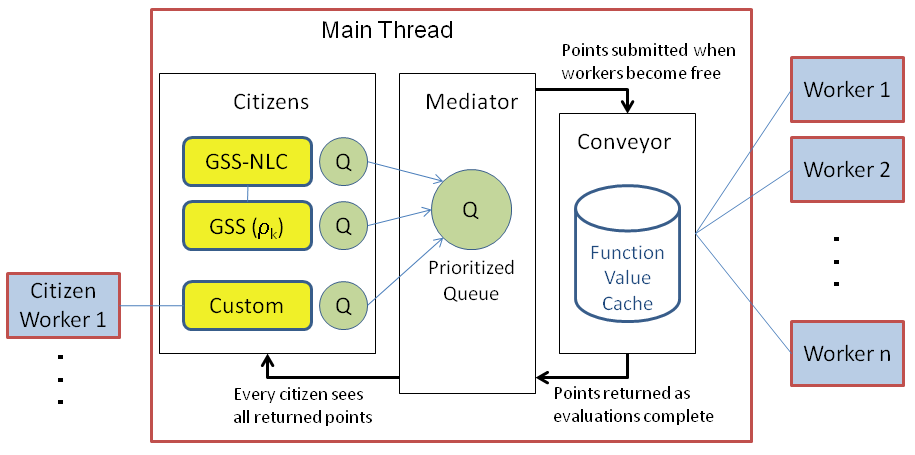
\includegraphics[width=5.8in]{BlockDiagram.png}
  \vspace{-5mm}
  \caption{HOPSPACK architecture diagram.}
  \label{fig:block-diagram}
\end{figure}

The Mediator runs a main processing loop until deciding that HOPSPACK should
stop.
Each Mediator iteration assembles trial point requests from all Citizens and
passes them to the Conveyor.  The Conveyor checks if new points can be fulfilled
from a cache, and sends the rest to idle workers for evaluation.  Two caches
are checked: a primary Cache of completed evaluations, and a Pending Cache
that lists trial points currently assigned to evaluation workers.
The Conveyor collects results from workers that have completed and passes
these back to the Mediator.
Citizens are then given the full set of newly evaluated points.  They examine
values and submit new trial points, which starts the
next iteration.  Citizens can also spawn dynamic ``child citizens'' to solve
subproblems.

From a citizen's point of view trial points are evaluated asynchronously,
so requests are typically managed with an internal queue, as shown in
\FIGREF{fig:block-diagram}.
The citizen submits trial points and may receive evaluated results at any
future iteration.  Evaluated points follow the order given from the citizen's
queue of trial points.  The citizen has the opportunity to retract previously
submitted points if they are still waiting on the Conveyor (for example,
the GSS citizen will retract old unevaluated requests when a new ``best point''
is found).
The Mediator collects trial requests from each citizen into a single
queue, interleaving points based on citizen priorities.

\FIGREF{fig:block-diagram} shows three citizen instances running
simultaneously.  The top two are connected because the GSS-NLC instance
dynamically created the GSS instance to solve a subproblem.  The citizen
labeled DIRECT has a parallel processing worker because its algorithm requires
significant CPU time to process points.  The ``citizen worker'' allows the
Mediator loop to run more quickly, and thus avoids slowing down other citizens.

As coordinator of the ``town'' of citizens, the Mediator decides when to
stop HOPSPACK and what final solution to return.
Each citizen decides when it has converged to a solution point, as defined by
its own criteria.  If all citizens have converged not necessarily to the same
point), then the Mediator stops.  It reports the best feasible point that it
has seen, regardless of which citizen generated the point.
If a problem-specific stop rule is supplied (for example,
an {\tt Objective Target} value, see \PGREF{param:PD-objtgt}),
then the Mediator will stop as soon as it sees a point satisfying the criteria
(see \SECREF{substoptest}).
The Mediator will also stop execution if a defined resource limit is reached
(for instance, execution time or the total number of worker evaluations).

The Cache in \FIGREF{fig:block-diagram} is an important feature of
HOPSPACK that often improves performance of GSS and related algorithms.
The Cache remembers all points and values that have been evaluated.  If a new
trial point is sufficiently close to a cached value, then it reports the stored
value instead of making another evaluation.  The definition of ``closeness''
is controlled by the
{\tt Cache Comparison Tolerance} parameter~(\PGREF{param:MD-cachetol}).
The Cache can also write its contents to a file
({\tt Cache Output File},~\PGREF{param:MD-cacheoutfile}), and load from
a file ({\tt Cache Input File},~\PGREF{param:MD-cacheinfile})
when HOPSPACK initializes.
This feature allows HOPSPACK to be interrupted without losing work.
As an interesting exercise, try solving a problem and saving the cache to a file,
and then solving again after initializing from the cache file.
If the Mediator is instructed to use
{\tt Synchronous Evaluations}~(\PGREF{param:MD-synch}), then the problem
will solve completely from cached information.
If not synchronous then there may be a few new iterations that choose different
directions, but the citizen should quickly build up a cache that can
solve without any evaluations.

Workers run copies of the application to collect objective and nonlinear
constraint values at trial points.  Each worker runs a HOPSPACK Evaluator
instance, which typically calls the application as a separate process for
each trial point.  See \SECREF{sec:calleval} for details on how an application
is called.
The workers on the right side of \FIGREF{fig:block-diagram} run in
parallel under direction of the Conveyor.  The Conveyor uses an Executor
subclass, specialized either for MPI or multithreaded (MT) operation, to
coordinate workers.
\FIGREF{fig:evalMPI} shows an example of the worker partitioning for
HOPSPACK using MPI on three nodes, and \FIGREF{fig:evalMT} shows an
example of worker partitioning for HOPSPACK using multithreading on a
quad-core machine.


MPI and MT are complementary methods of obtaining parallel
performance.  MPI-based HOPSPACK can solve problems on computing clusters with
tens of thousands of nodes, while MT exploits the multi-core capacity of
a single machine.  MT binaries are available for most platforms, but 
MPI requires recompiling HOPSPACK source code with an
MPI-aware compiler.  


\clearpage
\begin{figure}[!h]
  \begin{center}
    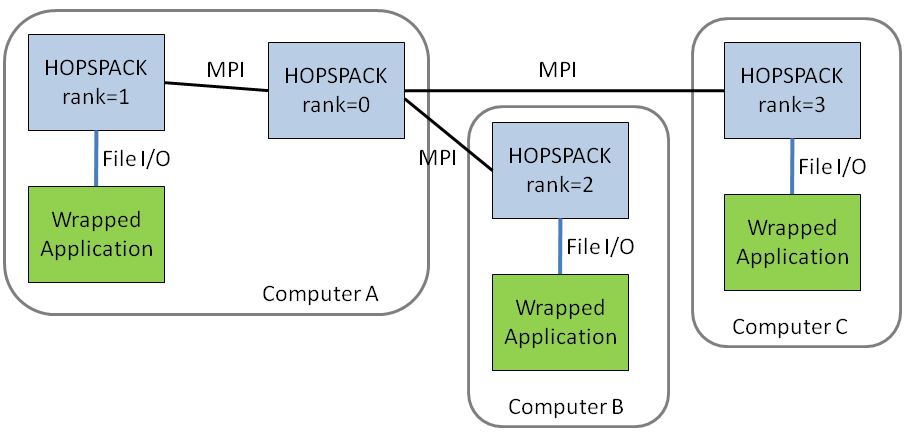
\includegraphics[width=5.0in]{EvalWithMpiClipped.png}
  \end{center}
  \vspace{-5mm}
  \caption{HOPSPACK communication using MPI.}
  \label{fig:evalMPI}
\end{figure}

\vspace{-11pt}
\noindent
In this example three copies of the application run in parallel
on three different computers.  Four MPI nodes are employed.
Evaluator nodes (rank 1, 2, 3) make system calls to the application,
and the main node (rank 0) runs the HOPSPACK Executor to control evaluations. 
The Mediator and Citizen solvers also run on the main node.
Execution may be faster if the main node can be placed on a separate computer.


% ADD SPACE TO LOOK BETTER, AND SO THE FIGURES CONSUME THE WHOLE PAGE.
% PUTTING \clearpage AT THE BOTTOM IS NOT THE SAME.
\vspace{11pt}
\vspace{11pt}
\vspace{11pt}


\begin{figure}[!h]
  \begin{center}
    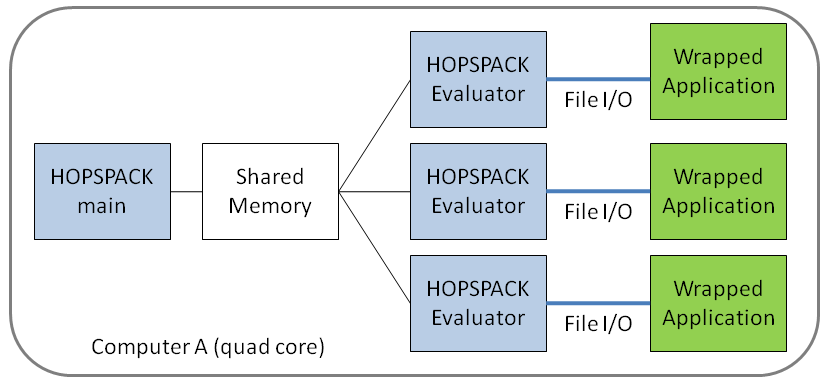
\includegraphics[width=5.0in]{EvalWithMtClipped.png}
  \end{center}
  \vspace{-5mm}
  \caption{HOPSPACK communication using multithreading.}
  \label{fig:evalMT}
\end{figure}

\vspace{-11pt}
\noindent
In this example three copies of the application run in parallel
as different processes on the same machine.  Four threads run in
the HOPSPACK process.
Evaluator threads make system calls to the application, and a fourth
thread runs the Executor to control evaluations.
The Mediator and Citizen solvers also run on the main thread.
Execution may be faster if additional cores are available for the application
instances.


%%%%%%%%%%%%%%%%%%%%
\subsection{Stopping Tests}
\label{substoptest}

The Mediator decides when to stop HOPSPACK and what to return as the best point
found.  The Mediator examines all evaluated points, regardless of which solver
submitted it, and keeps the best according to criteria discussed below.
HOPSPACK stops if any of the following conditions are met:
\begin{itemize}
  \item  All Citizen solvers are finished.
  \item  The total number of evaluations exceeds parameter
         {\tt Maximum Evaluations}~(\PGREF{param:MD-maxeval}).
         The default value of this parameter imposes no limit on evaluations.
  \item  The best point is feasible and satisfies an objective target set
         by the user.  Parameters
         {\tt Objective Target}~(\PGREF{param:PD-objtgt}) and
         {\tt Objective Percent Error}~(\PGREF{param:PD-objpcnt}) are
         used to set target values.  This is only useful if a practical value
         for the objective function is known.
\end{itemize}

A trial point is feasible if it satisfies the bound constraints, linear
constraints, and nonlinear constraints defined for the optimization problem.
Different tolerances are applied for each type of constraint:
\begin{INDENTdescription}
  \item[Bound constraints.]
    Variables are feasible if they satisfy the bound constraint exactly.
  \item[Linear constraints.]
    Linear equalities and inequalities are satisfied if within a tolerance set
    by parameter {\tt Active Tolerance} in the ``Linear Constraints'' sublist
    (\PGREF{param:LC-acttol}).  Computations are made in scaled coordinates
    (see {\tt Scaling}~(\PGREF{param:PD-scaling})) and normalized using
    the $L_2$ norm of the variables and the constraint.
  \item[Nonlinear constraints.]
    Nonlinear equalities and inequalities are satifisfied within a tolerance
    set by parameter {\tt Nonlinear Active Tolerance} in the
    ``Problem Definitions'' sublist (\PGREF{param:PD-nacttol}).
    Computations are not scaled.
\end{INDENTdescription}

The Mediator is responsible for choosing the best point that is output when
HOPSPACK finishes.  This is usually the same ``best point'' found by GSS
and other solvers, but not always.  The Mediator first seeks a point that
passes the feasibility tests described above.  If a feasible point has not
been found, then the least infeasible is ``best'', as measured by the
unscaled $L_{\infty}$ norm of the constraint vector.  If a feasible point has
been found, then a ``better'' point must pass the feasibility test and improve
on the objective value.
Source code is located in {\sf HOPSPACK\_Mediator.cpp} in the method
{\tt Mediator::updateBestPoint\_()}.

%TBD multiple objectives?


%%%%%%%%%%%%%%%%%%%%
\subsection{GSS Overview}
\label{subgss}

Generating Set Search (GSS) in HOPSPACK is an asynchronous implementation
of pattern search ideas.  An excellent review of pattern search methods
and convergence theory is in \cite{SIAMRev-KoLeTo03}.
GSS with linear constraints is explained in \cite{GSS-GrKoLe08} and
\cite{GSS-KoLeTo06},
and GSS with nonlinear constraints in \cite{GSS-GrKoSAND07}.
This overview will provide only a brief outline of the GSS algorithm.

The most basic GSS method addresses problems with continuous variables and
only bound constraints.  GSS begins with an arbitrary initial point and
iterates until stopped.  Each iteration generates a trial point along the
positive and negative direction of each coordinate axis.  The set of search
directions are centered on the current best point (called the ``parent'' point)
and initially extend a certain fixed distance.
If one of these trial points improves
on the parent, then it becomes the new best point for the next round.
If a trial point does worse, then the step size in that direction is reduced
to generate a replacement trial point.  GSS ends when the step length becomes
sufficiently short in every direction emanating from the current best point.
Details of this process are explained in the references and in
\SECREF{subconfig:GS}.  In particular, parameter
{\tt Step Tolerance}~(\PGREF{param:GS-steptol}) determines the length of
a ``sufficiently short'' step that stops the algorithm.

The HOPSPACK implementation of GSS is asynchronous in the sense that iterations
do not wait for all trial points in a direction set to be evaluated.  The
algorithm takes action on any partial set of results and is therefore ideal
for parallel architectures.  Convergence properties are no different for the
asynchronous algorithm.  An asynchronous implementation is especially tolerant
of applications whose run time varies based on the trial point.  For example,
if certain input regions require much more computation time in the application,
GSS will make progress in regions that run fast while waiting for the slower
points to evaluate.

GSS can respond to ``oracle'' inputs provided by another solver.  If an
evaluation result is better than the current GSS best point, then GSS will
adopt this as the new best point and begin searching around it.
The feature is controlled by parameter
{\tt Ignore Other Points}~(\PGREF{param:GS-ignore}).

The addition of linear constraints requires the set of directions to conform
with active constraints.  GSS honors linear equality constraints
at all times, and designates linear inequalities as active if the parent
point is within a distance {\tt Epsilon Max}~(\PGREF{param:GS-epsmax}).
Trial points are always feasible with respect to linear constraints.
To speed up the search, GSS can guess whether a nearby linear inequality
is active and ``snap'' a trial point to the bound; this feature is controlled
by parameters {\tt Snap To Boundary}~(\PGREF{param:GS-snap}) and
{\tt Snap Distance}~(\PGREF{param:GS-snapdist}).

{\bf GSS-NLC.}
The basic GSS solver handles continuous variables with bounds and linear
constraints, and was available in APPSPACK 5.0.  GSS is extended in HOPSPACK
to handle nonlinear constraints in a citizen called GSS-NLC.
The algorithm treats violations of nonlinear
constraints with a penalty term in the objective \cite{GSS-GrKoSAND07}.
An outer loop of iterations sets the weight of the penalty term and starts
a basic GSS citizen to solve a version of the problem without nonlinear
constraints.  This continues until the subproblem returns a feasible point
that also satisfies the {\tt Step Tolerance}~(\PGREF{param:GS-steptol}).
The inner loop of points generated by the subproblem solver behaves the same
as a basic GSS citizen except its initial point and stop criteria are set
by the GSS-NLC outer solver.

Performance of GSS-NLC can be heavily influenced by the penalty term and its
weight (the weight is also referred to as the penalty parameter).
Configuration parameters described in \SECREF{subconfig:GSN} provide
more information.
The values of {\tt Final Step Tolerance}~(\PGREF{param:GSN-finalstep}),
{\tt Nonlinear Active Tolerance}~(\PGREF{param:PD-nacttol}),
and {\tt Penalty Parameter Increase}~(\PGREF{param:GSN-penincrease})
are particularly important.  In general the penalty parameter should be increased
rapidly to force feasibility, but on some problems a slightly infeasible path
will reach an active nonlinear inequality constraint faster; in this case
the penalty parameter should be increased slowly.  The user is encouraged
to experiment.

The HOPSPACK framework allows a GSS-NLC citizen to create and manage subproblems
as separate GSS citizens.  This is shown schematically in
Figure~\ref{fig:block-diagram}, where a GSS-NLC citizen is connected with
a citizen labelled GSS($\rho_k$) (the penalty parameter of the subproblem
is $\rho_k$).  Subproblems run like any other citizen, but when they finish
their result is returned to the parent citizen that created them.
This idea is leveraged to extend GSS for problems with integer variables
and multiple start points.


\begin{figure}[!ht]
  \begin{center}
    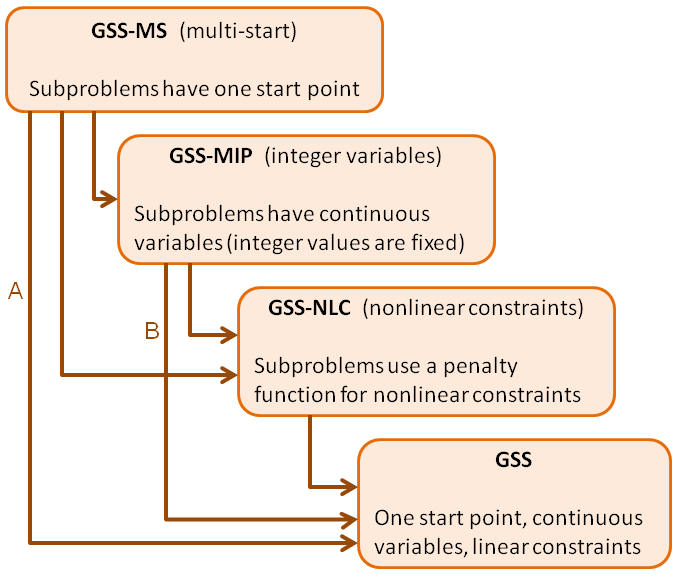
\includegraphics[width=5.0in]{GssHierarchyDiagram.png}
    \vspace{-5mm}
  \caption{Hierarchy of GSS algorithms,
           showing how complicated problems are decomposed into
           simpler subproblems.
           Arrows ``A'' and ``B'' are referenced in the text.
          }
  \label{fig:gss-hier}
  \end{center}
\end{figure}

\FIGREF{fig:gss-hier} shows how a notional family of GSS algorithms can address
a hierarchy of problem types.  (The current HOPSPACK release does not include
GSS-MIP, and GSS-MS has only partial functionality.)
Complicated problems at the top follow one or more
arrows to reach the basic GSS building block at the bottom.  An arrow indicates
that a problem is transformed into a sequence of simpler subproblems.
For example, path {\it A} shows that a multi-start problem with continuous
variables and linear constraints is solved by creating GSS subproblems, each
with a different starting point.  The parent GSS-MS collects subproblem results
and generates new start points until finished.
Path {\it B} shows that a problem with integer-valued variables and linear
constraints can be solved by creating GSS subproblems, each treating integer
variables as fixed to a specific integer value.  The parent GSS-MIP follows
a branching tree or other combinatorial strategy to decide how to fix
integer variables in each subproblem.
In the most complex case, a problem with multiple start points,
integer variables, and nonlinear constraints would cascade from GSS-MS
to GSS-MIP to GSS-NLC to GSS, creating subproblems of every type.
